% ---------------------------------------------------------------------------- %
\section{Linguometer architecture}
\label{ch:linguometer:architecture}
% ---------------------------------------------------------------------------- %
The mechanisms underlying the Linguometer setup could be fairly complex to
describe since most of the instrumentation used is
not specifically designed with simultaneous recordings in mind.
Furthermore, just a part of the synchronization is done in hardware; 
data alignment, segmentation and correction is done in post-processing.
As a result, synchronization is not ``one-shot'', and in order to describe the
whole process clearly, a bottom-up approach is used.
Once we have covered a few critical technical issues, the
description will follow a more classical top-down approach.
At the end of this Section the synchronization mechanism should be clear and 
the reader should be able to understand how and why the data-streams are routed
through particular paths. 
% ---------------------------------------------------------------------------- %
%%\subsection{Building blocks}
\label{sec:linguometer:architecture:blocks}
% ---------------------------------------------------------------------------- %
Figure~\ref{fig:linguometer:architecture:schematics} shows the complete
Linguometer block diagram.
In order to provide a straightforward description of the Linguometer, each
single block is considered in turn, describing the input/output data formats.
Furthermore, each block is to be considered as a ``meta-block'' since each
device is described with some degree of abstraction.
% ---------------------------------------------------------------------------- %
\subsection{Recording instrumentation}
% ---------------------------------------------------------------------------- %
% ---------------------------------------------------------------------------- %
\begin{figure}
	\centering
	  \subfigure[\label{fig:linguometer:architecture:bb:instruments:ag}]
		{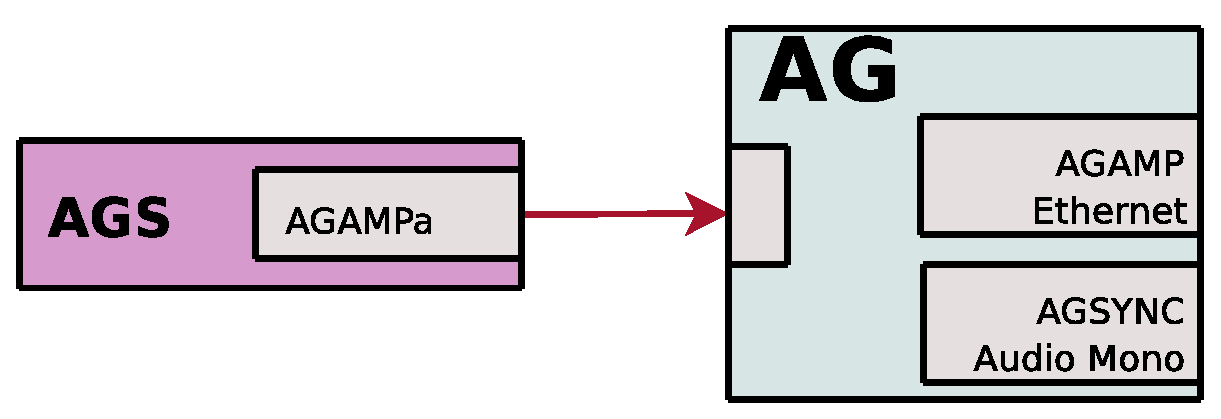
\includegraphics[width=0.45\textwidth]{include/linguometer/images/bb_ag.eps}}
		\hspace{0.05\textwidth}
	  \subfigure[\label{fig:linguometer:architecture:bb:instruments:us}]
		{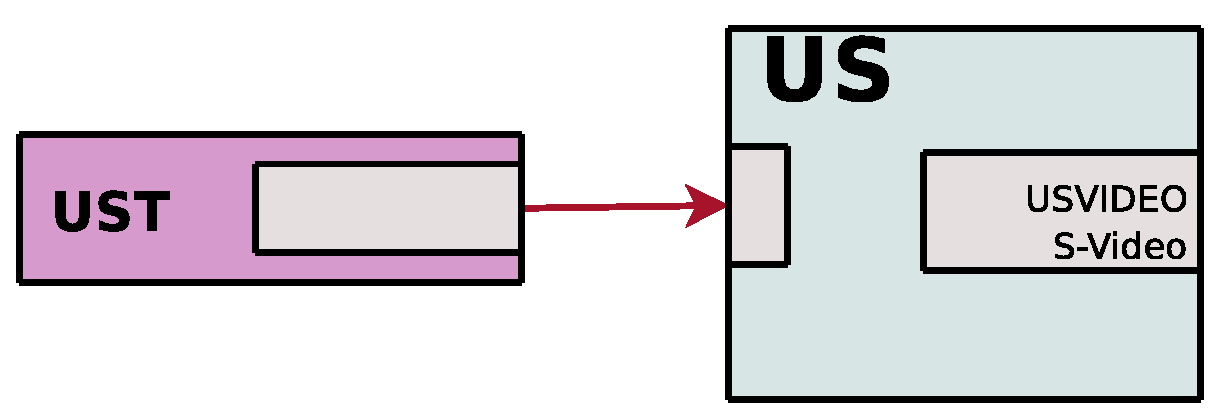
\includegraphics[width=0.45\textwidth]{include/linguometer/images/bb_us.eps}}

	  \subfigure[\label{fig:linguometer:architecture:bb:instruments:lg}]
		{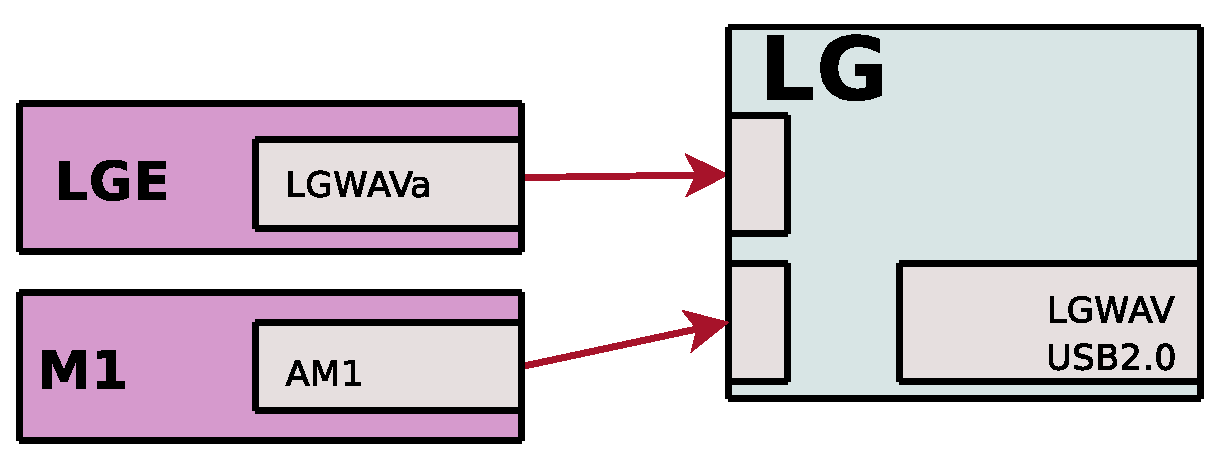
\includegraphics[width=0.45\textwidth]{include/linguometer/images/bb_lg.eps}}
		\hspace{0.05\textwidth}
	  \subfigure[\label{fig:linguometer:architecture:bb:instruments:cc}]
		{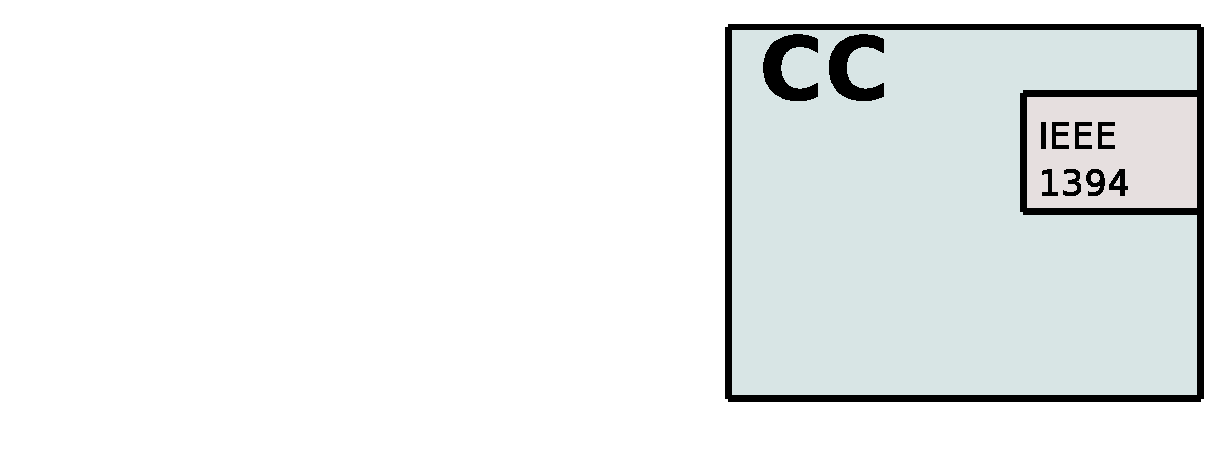
\includegraphics[width=0.45\textwidth]{include/linguometer/images/bb_cc.eps}}

	\caption[Building blocks: instrumentation]{\textbf{Building blocks:
	instrumentation}: (a) articulograph, (b) ultrasound system,
	(c) laryngograph and (d) camcorder.}
	\label{fig:linguometer:architecture:bb:instruments}
\end{figure}
% ---------------------------------------------------------------------------- %

Figure~\ref{fig:linguometer:architecture:bb:instruments} shows the recording
instrumentation: the laryngograph (\sig{LG}), the articulograph (\sig{AG}) and
the ultrasound system (\sig{US}).
%
Two sensing devices are connected to the \sig{LG} block: the laryngograph
electrodes \sig{LGE} and the Shure SM58 microphone \sig{M1}.
The \sig{LG} device acquires and digitizes both the analog EGG signal
\sig{LGWAVa} and the analog audio signal \sig{AM1}.
After AD conversion (PCM Stereo, 16bit, 22.5 kHz), the signals are transmitted
to the instrumentation control computer (\sig{PC1}) via an USB 2.0 interface. 
The right channel of \sig{LGWAW} contains the digitized \sig{LGWAVa} EGG 
signal sensed via \sig{LGE}, while the left channel contains the digitized
speech signal acquired via \sig{M1} (Figure~\ref{fig:linguometer:lg:example}).

A single sensing meta-device is connected to the \sig{AG} block, that is
\sig{AGS}.
The term ``meta-device'' provides a sufficient level of abstraction for the
physical representation of the twelve articulograph sensors.
The \sig{AG} block communicates via TCP/IP with the instrumentation control
computer \sig{PC1} via the \sig{AGAMP} Ethernet interface.
As a matter of fact, \sig{AG} acquires and digitizes the analog amplitudes
\sig{AGAMPa}, then transmits the acquired data to the control PC via the 
\sig{AGAMP} interface by means of TCP/IP.
The \sig{AGAMP} data sampling rate is 200 Hz and the dimensionality is equal to 
72. In fact, 12 is the number of sensors and 6 is the number of reference coils.
Since each coil induces, via a generated EM field, a current on each sensor, the
total number of current amplitudes is equal to $12\times6 = 72$.
The \sig{AGAMP} interface is not used just to send data. 
In fact, it is also used by
the articulograph control software (running on \sig{PC1}) to transmit
control instructions.
When the experimenter decides to start or stop a recording session, an analog 
synchronization signal is generated by the Sybox-Opto4 synchronization device.
The synchronization signal, represented in the Linguometer schematic with
the \sig{AGSYNC} label\footnote{The Sybox-Opto4 device can route the
synchronization signal to a total of four instruments 
(Section~\ref{sec:linguometer:instrumentation:ag}). The synchronization
signal is electronically replicated on four serial port connectors (DE-9).}, 
consists in a peak that reach saturation. In this context, a positive saturation
peak highlights the beginning of a recording session, while a negative
saturation peak indicates the session's end.
%The synchronization signal that represents the beginning of a recording session
%differs from the one that represents the ending of a recording session.

The ultrasound system block (\sig{US}) receives a single input from the
ultrasound system transducer (\sig{UST}) via a dedicated and proprietary
interface. The \sig{US} block is routed to a standard VGA monitor via a D-SUB
connection (not shown). 
The same video signal that is used to refresh the monitor is available on
an S-Video connector, in standard PAL format ($720\times576$ pixels, 25 frames
per second, interlaced).
As said in the previous section, Toshiba provided also a RAW module. 
The RAW data recordings are not compliant with the workflow required by the
Linguometer recordings; for this reason the Linguometer uses the S-Video
signal (\sig{USVIDEO}) to acquire the 
ultrasonographic data.

The camcorder (\sig{CC}) is the last recording device to be discussed in this
Section.
The camcorder operates as a stand-alone device, that means that it records
both audio and video data temporarily in an internal MiniDV tape.
Once the recording session is over, the camcorder is connected to the caching
server (\sig{PC2}) via a standard IEEE-1394 interface and the audio/video
stream is stored on the hard drive in a standard DVSD container.
The camcorder data format consists of a video track of facial expressions (YUV2,
$720\times576$ pixels, 25 frames per second) and a stereo audio track 
of the speech signal (PCM Stereo, 16 bit, 48 kHz).
% ---------------------------------------------------------------------------- %
\subsection{Setup-control computers}
% ---------------------------------------------------------------------------- %
A total of four computers are used to control the Linguometer setup.
Each computer is customized to run a specific task, such as instrumentation 
control (\sig{PC1}), stimuli presentation and segmentation-signal routing 
(\sig{PC0}), data-caching and backup (\sig{PC2}) and finally, setup-control 
(\sig{PC3}).
Figure~\ref{fig:linguometer:architecture:bb:pc} shows the corresponding blocks
in the Linguometer schematic.
% ---------------------------------------------------------------------------- %
\begin{figure}
	\centering
	  \subfigure[\label{fig:linguometer:architecture:bb:pc:2}]
		{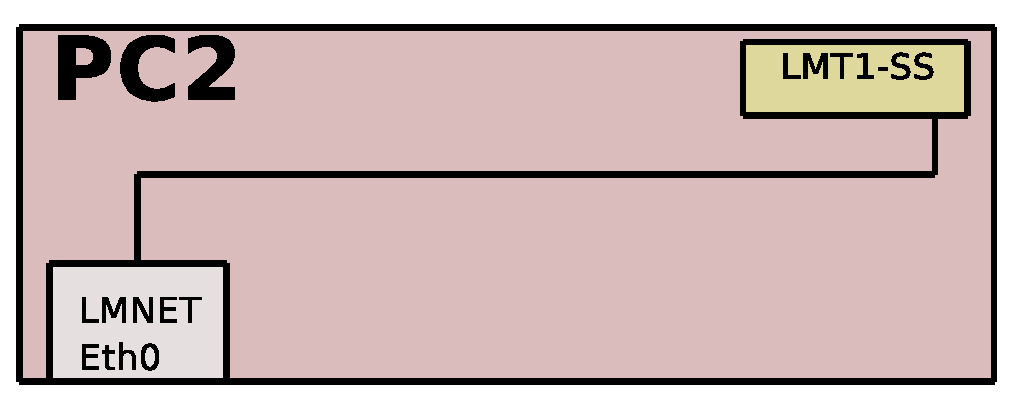
\includegraphics[width=0.45\textwidth]{include/linguometer/images/bb_pc2.eps}}
		\hspace{0.05\textwidth}
	  \subfigure[\label{fig:linguometer:architecture:bb:pc:3}]
		{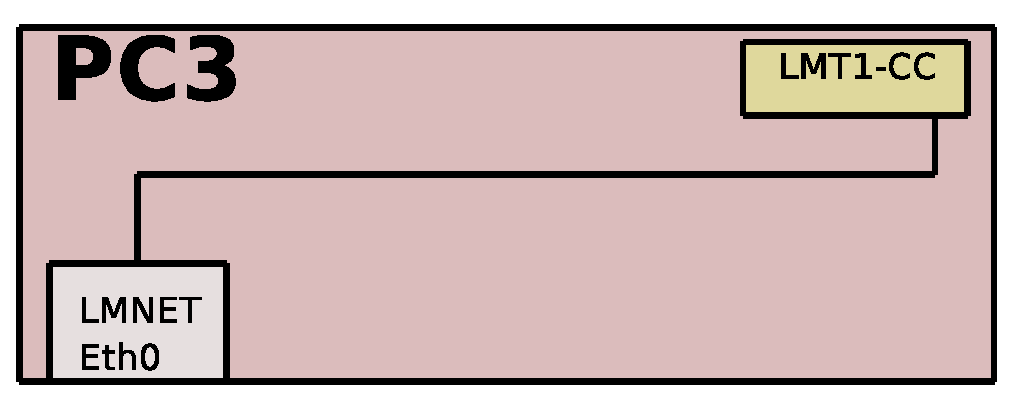
\includegraphics[width=0.45\textwidth]{include/linguometer/images/bb_pc3.eps}}

		\subfigure[\label{fig:linguometer:architecture:bb:pc:1}]
		{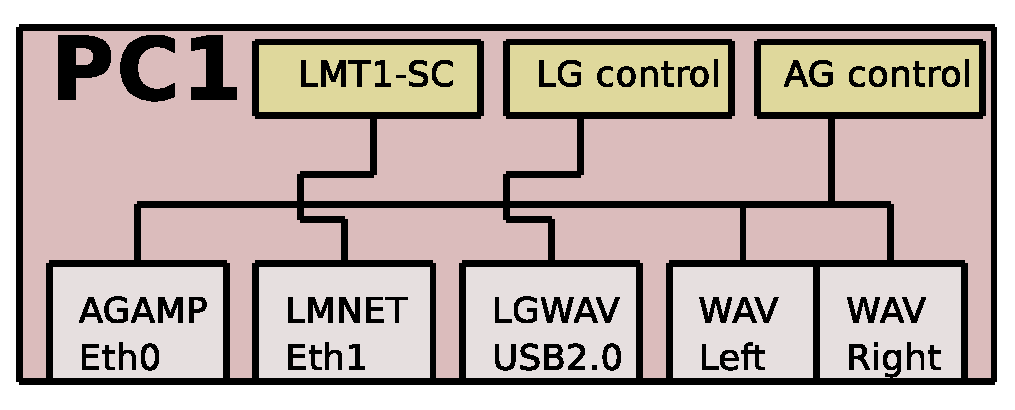
\includegraphics[width=0.45\textwidth]{include/linguometer/images/bb_pc1.eps}}
		\hspace{0.05\textwidth}
	  \subfigure[\label{fig:linguometer:architecture:bb:pc:0}]
		{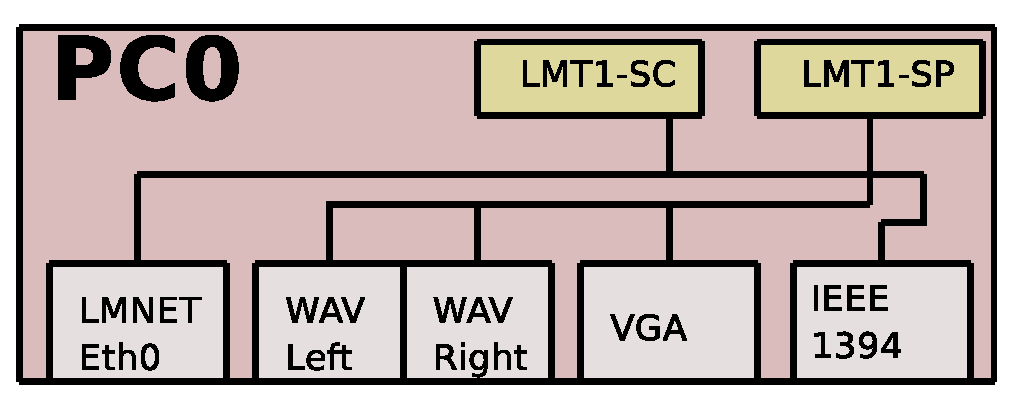
\includegraphics[width=0.45\textwidth]{include/linguometer/images/bb_pc0.eps}}

	\caption[Building blocks: setup-control computers]{\textbf{Building blocks: setup-control computers}: (a) data-caching server \sig{PC2}, (b) setup-control notebook  \sig{PC3}, (c) instrumentation-control workstation \sig{PC1} and (d) stimuli presentation and segmentation-signal routing workstation \sig{PC0}.}
	\label{fig:linguometer:architecture:bb:pc}
\end{figure}
% ---------------------------------------------------------------------------- %


The instrumentation-control software runs on \sig{PC1} (Microsoft Windows XP
Professional).
The computer is equipped with two Ethernet cards: \sig{Eth0} and \sig{Eth1}.
The first interface is connected with a crossed RJ45 100Mbps cable to the
articulograph \sig{AG}.
The \sig{AG control} software sends control messages to \sig{AG} and receives
the \sig{AGAMP} data.
When the experimenter starts a recording sweep, \sig{AG control} starts reading
the data sent by \sig{AG}. Once the TCP/IP connection is established and the
data transmission is started, \sig{AG} generates via the Sybox-Opto4
synchronization device the analog synchronization signal \sig{AGSYNC}.
\sig{AGSYNC} is routed to the left channel of the Line-In connector of a 
Creative Audigy sound card (\sig{WAV L-IN}).
The Shure SM7B microphone (\sig{M0}) sense the speech signal and transduce it
into the analog signal \sig{AM0}.
The \sig{AM0} signal is routed to a mixer and then to an audio/video
acquisition card (\sig{AMX} and \sig{ACC} respectively), and then reaches the 
right channel of the Line-In connector of the \sig{PC1} sound card
(\sig{WAV R-IN}).
The motivations for the two-stages routing of the \sig{AM0} signal are
described later on this Section, since this particular solution constitutes part
of the synchronization mechanism core.
In this context it is important to understand that \sig{AG control}, once 
the \sig{AGSYNC} signal is detected, starts recording the \sig{AGAMP} data and
a speech signal that results from the mixing of the \sig{AM0} signal with
particular segmentation signals generated by \sig{PC0}.
The speech signal\footnote{The speech signal recorded by \sig{AG} (PCM, 16 bit,
16 kHz) will be referred as \sig{AGWAV}.} and the \sig{AGAMP} data are recorded
synchronously (Section~\ref{sec:linguometer:instrumentation:ag}) and stored on
the data-caching server \sig{PC2} using an \emph{LMTools1} Perl script
(\sig{LMT1-SC}).
The second Ethernet connection connects \sig{PC1} to the \sig{LMNET} Class-C 
LAN (Local Area Network).
The \sig{LG control} software is used to acquire the previously described 
\sig{LGWAV} data.

The second workstation used in the recording room is \sig{PC0}. 
This host plays a crucial role in the synchronization mechanism, discussed in
Section~\ref{sec:linguometer:technical:signals}.
The synchronization mechanism, as already said, is not trivial and requires an
appropriate description. 
In this perspective, the role of \sig{PC0} is only partially described in this
paragraph.
\sig{PC0} runs the Gentoo Linux distribution, equipped with a low-latency
Linux Kernel (v2.6.18).
Figure \ref{fig:linguometer:architecture:bb:pc:0} shows the I/O devices used for
the Linguometer setup and the software modules that rely on such devices.\\
The \sig{LMT1-SP} software module refers to the \emph{lmwords}
stimuli-presentation program\footnote{All the programs/script with an
\emph{lm\_} prefix are part of the \emph{LMTools1} or \emph{LMTools2}
tool-kits.}. 
This program displays the stimuli (words and pseudo-words), on the LCD screen
connected to the \sig{VGA} interface.
Before and after the presentation of each word \emph{lmwords} generates a 
segmentation signal facilitating the post-processing segmentation task, as
shown in Section~\ref{sec:linguometer:technical:lmwords}.
The segmentation signal is routed from the \sig{PC0} ``Creative SoundBlaster 
Live'' sound card (\sig{WAV L-OUT} and \sig{WAV R-OUT}) to the mixer
(\sig{AMX}), and mixed with the \sig{AM0} speech signal.
Once the \sig{AM0} signal and the segmentation signals are mixed together, the
signal is routed through the acquisition card \sig{ACD} to \sig{PC1}, where
it is  recorded by the \sig{AG control} software (as discussed in the previous
paragraph).\\
As shown in Figure~\ref{fig:linguometer:architecture:bb:pc:0}, \sig{PC0} is also
equipped with an IEEE-1394 interface (\sig{IEEE 1394}), to which the 
\sig{ACD} acquisition card is connected. 
The \sig{ACD} card digitizes the \sig{USVIDEO} signal, the \sig{AM0} signal
mixed with the segmentation signals and the \sig{AGSYNC} synchronization signal.
\sig{PC0} acquires the stream and stores it (via \sig{LMT1-SC}) onto a network
drive shared by the data-caching server \sig{PC2}.
A standard DVSD container is used to store the signals digitized by \sig{ACD}.

The \sig{PC2} computer runs Gentoo Linux with a standard Linux Kernel (v2.6.18).
It shares on the \sig{LMNET} LAN a RAID1 point of storage to which the data is
streamed while it is being acquired.
The data is also copied on a backup device on the daily basis.
After an experiment has been recorded, the \sig{CC} camcorder is plugged into 
the \sig{PC1} \sig{IEEE 1394} interface and the audio/video stream of the facial
expressions is saved on the hard drive.
Finally, the \sig{PC3} notebook is used to monitor data acquisition and data 
transfer in real-time.
% ---------------------------------------------------------------------------- %
\subsection{Audio/Video routing and acquisition devices}
% ---------------------------------------------------------------------------- %
% ---------------------------------------------------------------------------- %
\begin{figure}
	\centering
	  \subfigure[\label{fig:linguometer:architecture:bb:routing:am}]
		{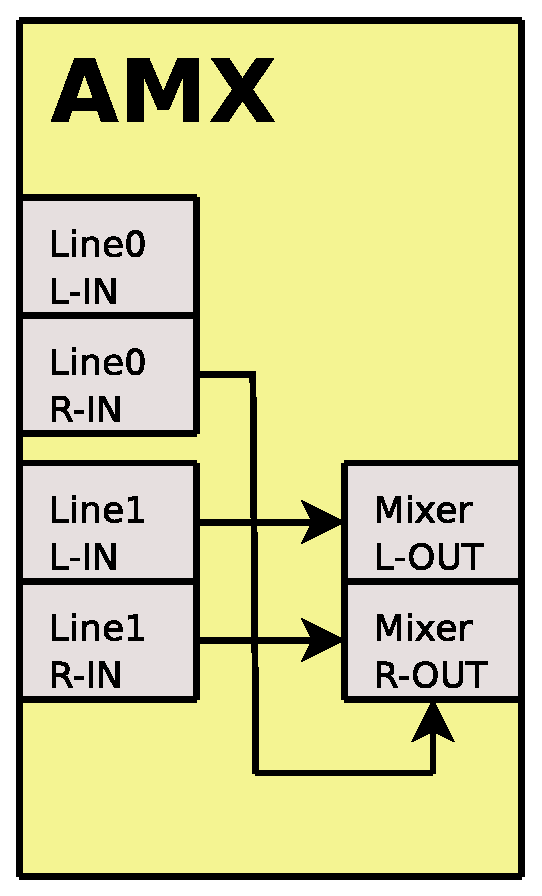
\includegraphics[width=0.25\textwidth]{include/linguometer/images/bb_am.eps}}
		\hspace{0.10\textwidth}
	  \subfigure[\label{fig:linguometer:architecture:bb:routing:ac}]
		{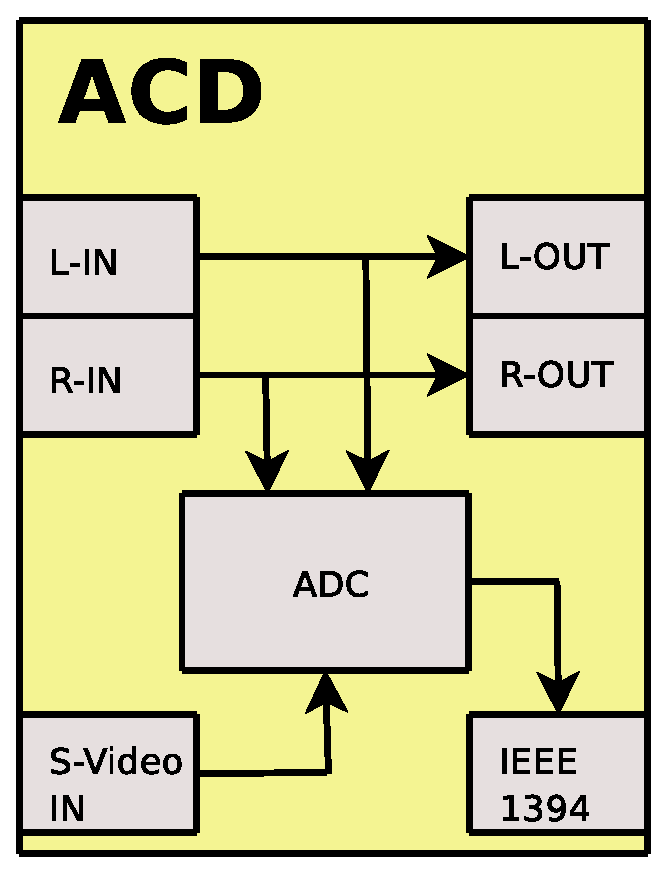
\includegraphics[width=0.25\textwidth]{include/linguometer/images/bb_ac.eps}}

	\caption[Building blocks: stream routing and acquisition]{\textbf{Building blocks:
	stream routing and acquisition}:
	.}
	\label{fig:linguometer:architecture:bb:routing}
\end{figure}
% ---------------------------------------------------------------------------- %

A total of two devices are used to route and acquire the audio/video signals:
the \sig{AMX} audio mixer by Behringher and the \sig{ACD} acquisition card by
Terratec (Section~\ref{ch:linguometer:instrumentation:av}).
Figure~\ref{fig:linguometer:architecture:bb:routing} shows the \sig{AMX} and the
\sig{ACD} blocks.

The \sig{AMX} mixer is supplied with two microphone inputs and two stereo
inputs.
For the sake of simplicity,  the \sig{AMX} block is shown as a device with 
two stereo inputs (\sig{Line0} and \sig{Line1}) and a stereo output
(\sig{Mixer}).
The \sig{Line0} input receives the stereo segmentation signal (generated by 
\emph{lmwords}) from \sig{PC0}.
The \sig{Line1} input receives the \sig{AM0} signal from \sig{M0} (right
channel \sig{Line1 R-IN}) and the synchronization signal \sig{AGSYNC} from 
the \sig{AG} articulograph (Left channel \sig{Line1 L-IN}).

The speech signal from \sig{M0} is mixed with the right channel of
the segmentation signal on \sig{Line0 R-IN}\footnote{Only the right channel of
the stereo segmentation signal carries useful information. For this reason,
just the right component is mixed with the speech signal on \sig{Line1 R-IN}.} 
and then is routed to \sig{Mixer R-OUT}. 
The synchronization signal \sig{AGSYNC} is directly routed to \sig{Mixer L-OUT}
and it is not mixed with any other signal, so it preserves the original
information.
The \sig{Mixer L-OUT} and the \sig{Mixer R-OUT} outputs are then routed to the
\sig{ACD} acquisition card, where they are synchronously digitized and then
acquired, via the \sig{IEEE 1394} interface, by \sig{PC0}.
The speech signal recorded by the acquisition card is then sent to \sig{PC1}
through the \sig{L-OUT} connector, and is recorded by the \sig{AG control}
software (as discussed earlier).
% ---------------------------------------------------------------------------- %
\subsection{Workflow and complete block diagrams}
\label{sec:linguometer:architecture:diagram}
% ---------------------------------------------------------------------------- %
Each building block included in the complete diagram
(Figure~\ref{fig:linguometer:architecture:schematics}) has been described in 
Section~\ref{sec:linguometer:architecture:blocks}, introducing
the logical relationships that exist between the whole set of blocks.
%The aim of this section is to present the Linguometer recording mechanism
%from a temporal point of view.
A small set of the connections among different blocks are recursive in the 
sense that  a single block (e.g.: \sig{PC0}) both sends and receives data 
to/from the same device (e.g.: the mixer \sig{AMX} and the acquisition 
card \sig{ACD}). This very last property of the Linguometer connections makes 
the description of the recording mechanism moderately complicated.
In this section the Linguometer workflow is introduced in order to bring the
whole explanation to a friendlier level.\\

The complete block diagram, the Linguometer schematic, describes the Linguometer
at the ``connection level'' and constitutes by itself an important source of
information, but does not completely describe the task of running
the Linguometer from a temporal perspective.
For this reason, we introduce the workflow diagram, shown
in Figure~\ref{fig:linguometer:architecture:workflow}, and use it as a
starting point to describe the whole synchronization process.
When needed, the description will jump back to the connection level, switching
from the higher-level abstraction to the lower-level physical connections.
Furthermore, it is important to specify that the term ``workflow'' refers to 
the set of operations performed by the
experimenters, such as starting/stopping a recording sweep with a particular 
device and presenting a stimulus.
%The reader may think that the chosen approach makes the description of
%each building block unnecessary.
%In reality, this is not the case.

After running few test experiments with an expert reference subject, it 
became clear that the Linguometer had to fit a crucial requirement, that is
the  duration of the experiments.
Although the recording-support devices (table, stool and stand,
Section~\ref{ch:linguometer:instrumentation:custom}) have been designed and 
built 
to provide a sufficient degree of compliance, the subjects started suffering
from the forced position after circa 45 minutes, becoming impatient and moving very
often. 
The subjects also reported that salivation increases during the experiment,
surely due to the fact that 9 out of 12 articulograph sensors were placed on the
tongue, lips and teeth.
If salivation increases, the subjects swallow more often, thus moving the
larynx. This kind of movement presses the
larynx against the ultrasonograpic transducer, inflicting pain on the subject.

As discussed later in this Section, the subjects had to read and utter circa 630
utterances (words and syllables: 70\% words, 30\% syllables), divided in 9 batches.
Recording such a large amount of stimuli requires the recording devices and
the recording software to be stable and to endow fast crash-recovery
capabilities.
%Furthermore, the recording workflow required
%stability and recovering
%capabilities. 
A quite poor example of those two qualities is provided by the Cartsens AG500
articulograph. 
In fact, not only did the control software (\sig{AG control}) 
keep crashing during the majority of the experiments (6 out of 9), but each 
software crash required the rebooting of both the control computer and the 
articulograph itself, thus losing precious time\footnote{Carstens 
Medizinelektronik GmbH is working on the new version of
the control and acquisition software. Details at: http://wiki.ag500.net/}. 
Moreover, the device crashed in an unpredictable
way (e.g.: while recording and/or while starting a recording session), so that
it was not possible to forestall the odd behavior.

A total of three key-words emerge from the preceding paragraphs: 
duration, stability and crash-recovery capabilities.
Recovering from software and hardware problems during the investigations proved
to be a quite complicated task for the experimenters and for the examined
subject.
Moreover, stability and crash-recovery capabilities both affect the duration
of an experiment. 
In this context, a well designed workflow protocol plays a very important role,
since it allows the experimenters to record easily and eventually to recover
from hardware and software failures without invalidating the whole experiment.

From a practical point of view, recording with the Linguometer requires
starting/stopping one half of the recording devices ``una tantum'', that is at
the beginning and at the end of the experiments respectively (e.g.: ultrasound 
system and
camcorder).
The remaining devices are started/stopped before and after each one of the 9
batches of stimuli (e.g.: articulograph and laryngograph).
The need to start/stop the acquisition arises from limitations at the
software level of the articulograph and the laryngograph.
In fact, the articulograph control software can record a maximum of 65000 
samples\footnote{Each ``sample'' is  72 values of current
amplitude (12 sensors, 6 reference coils).} at 200 Hz, and 
therefore the maximum
duration of the sweep is 325 seconds (circa 5 minutes and 25 seconds).
Similarly, the laryngograph control software supports a maximum of 10 minutes
for each recording, but this duration is still too short if compared to the
total duration of each experiment~(circa~35~minutes).

On the other hand, recording facial expressions with the camcorder and 
tongue motion with the ultrasound system is fairly simple.
The audio/video data recorded with the camcorder is immediately stored on a
MiniDV digital tape, and
%The experimenters used one-hour long MiniDV tapes
%for the Linguometer investigations.
one-hour long tapes usually fit perfectly the requirements.
In the same way, the ultrasound system video stream, the main speech signal
(the signal \sig{AM0} from the \sig{M0} microphone) mixed with the segmentation
signal and the synchronization signal generated by the articulograph
(\sig{AGSYNC}) are acquired using the \sig{ACD} acquisition card by \sig{PC0}
and immediately stored on a large hard drive shared on the network by \sig{PC2}.

The workflow diagram is subdivided into two main areas: workflow and
data-streams (Figure~\ref{fig:linguometer:architecture:workflow}).
The upper panel, workflow, illustrates the time instants in which the 
recording devices are started and stopped by the experimenters.
The lower area of the diagram, data-streams, shows a simplified representation
of the recorded streams.
Although the representation is symbolic, it perfectly shows how the
synchronization and the segmentation signals are used within the Linguometer.
Furthermore, the workflow and the data-stream areas share the same time scale.
A really simple experiment is described in
Figure~\ref{fig:linguometer:architecture:workflow}.
The subject is asked to read two words presented on the LCD screen used
for the experiments.
In this particular case, the batch of stimuli is really small (just 2 words),
but it is sufficient to describe the recording mechanism.
As previously said, real experiments involved 9 batches of 70 stimuli, resulting
in longer sequences.

In the workflow area, five bars are shown (\wf{CC}, \wf{US}, \wf{LG},
\wf{AG} and \wf{WD}): each one represents a particular time interval and a 
pair of time labels pinpoint its beginning and its end.
For example, the first bar (\wf{CC}) starts at \tstart{CC} and ends at 
\tstop{CC}.
It represents the interval of time in which the camcorder is recording facial 
expressions.
Similarly, \wf{US}, \wf{LG} and \wf{AG} represent the ultrasound system, the
laryngograph and the articulograph recording intervals respectively.
The \wf{WD} bar plays a special role in the workflow diagram.
Moreover, no recording device that resembles the \wf{WD} label has been
described in so far.
In fact, the \wf{WD} label symbolizes the stimuli-submission protocol, handled 
by \emph{lmwords} (Section~\ref{sec:linguometer:technical:lmwords}).
From the temporal perspective, \wf{WD} depicts the submission of a batch of 
stimuli with \wf{WD-0} and \wf{WD-1} being the 2 words used for the simplified
example.
% ---------------------------------------------------------------------------- %
\begin{sidewaysfigure}%[!ht]
\centering
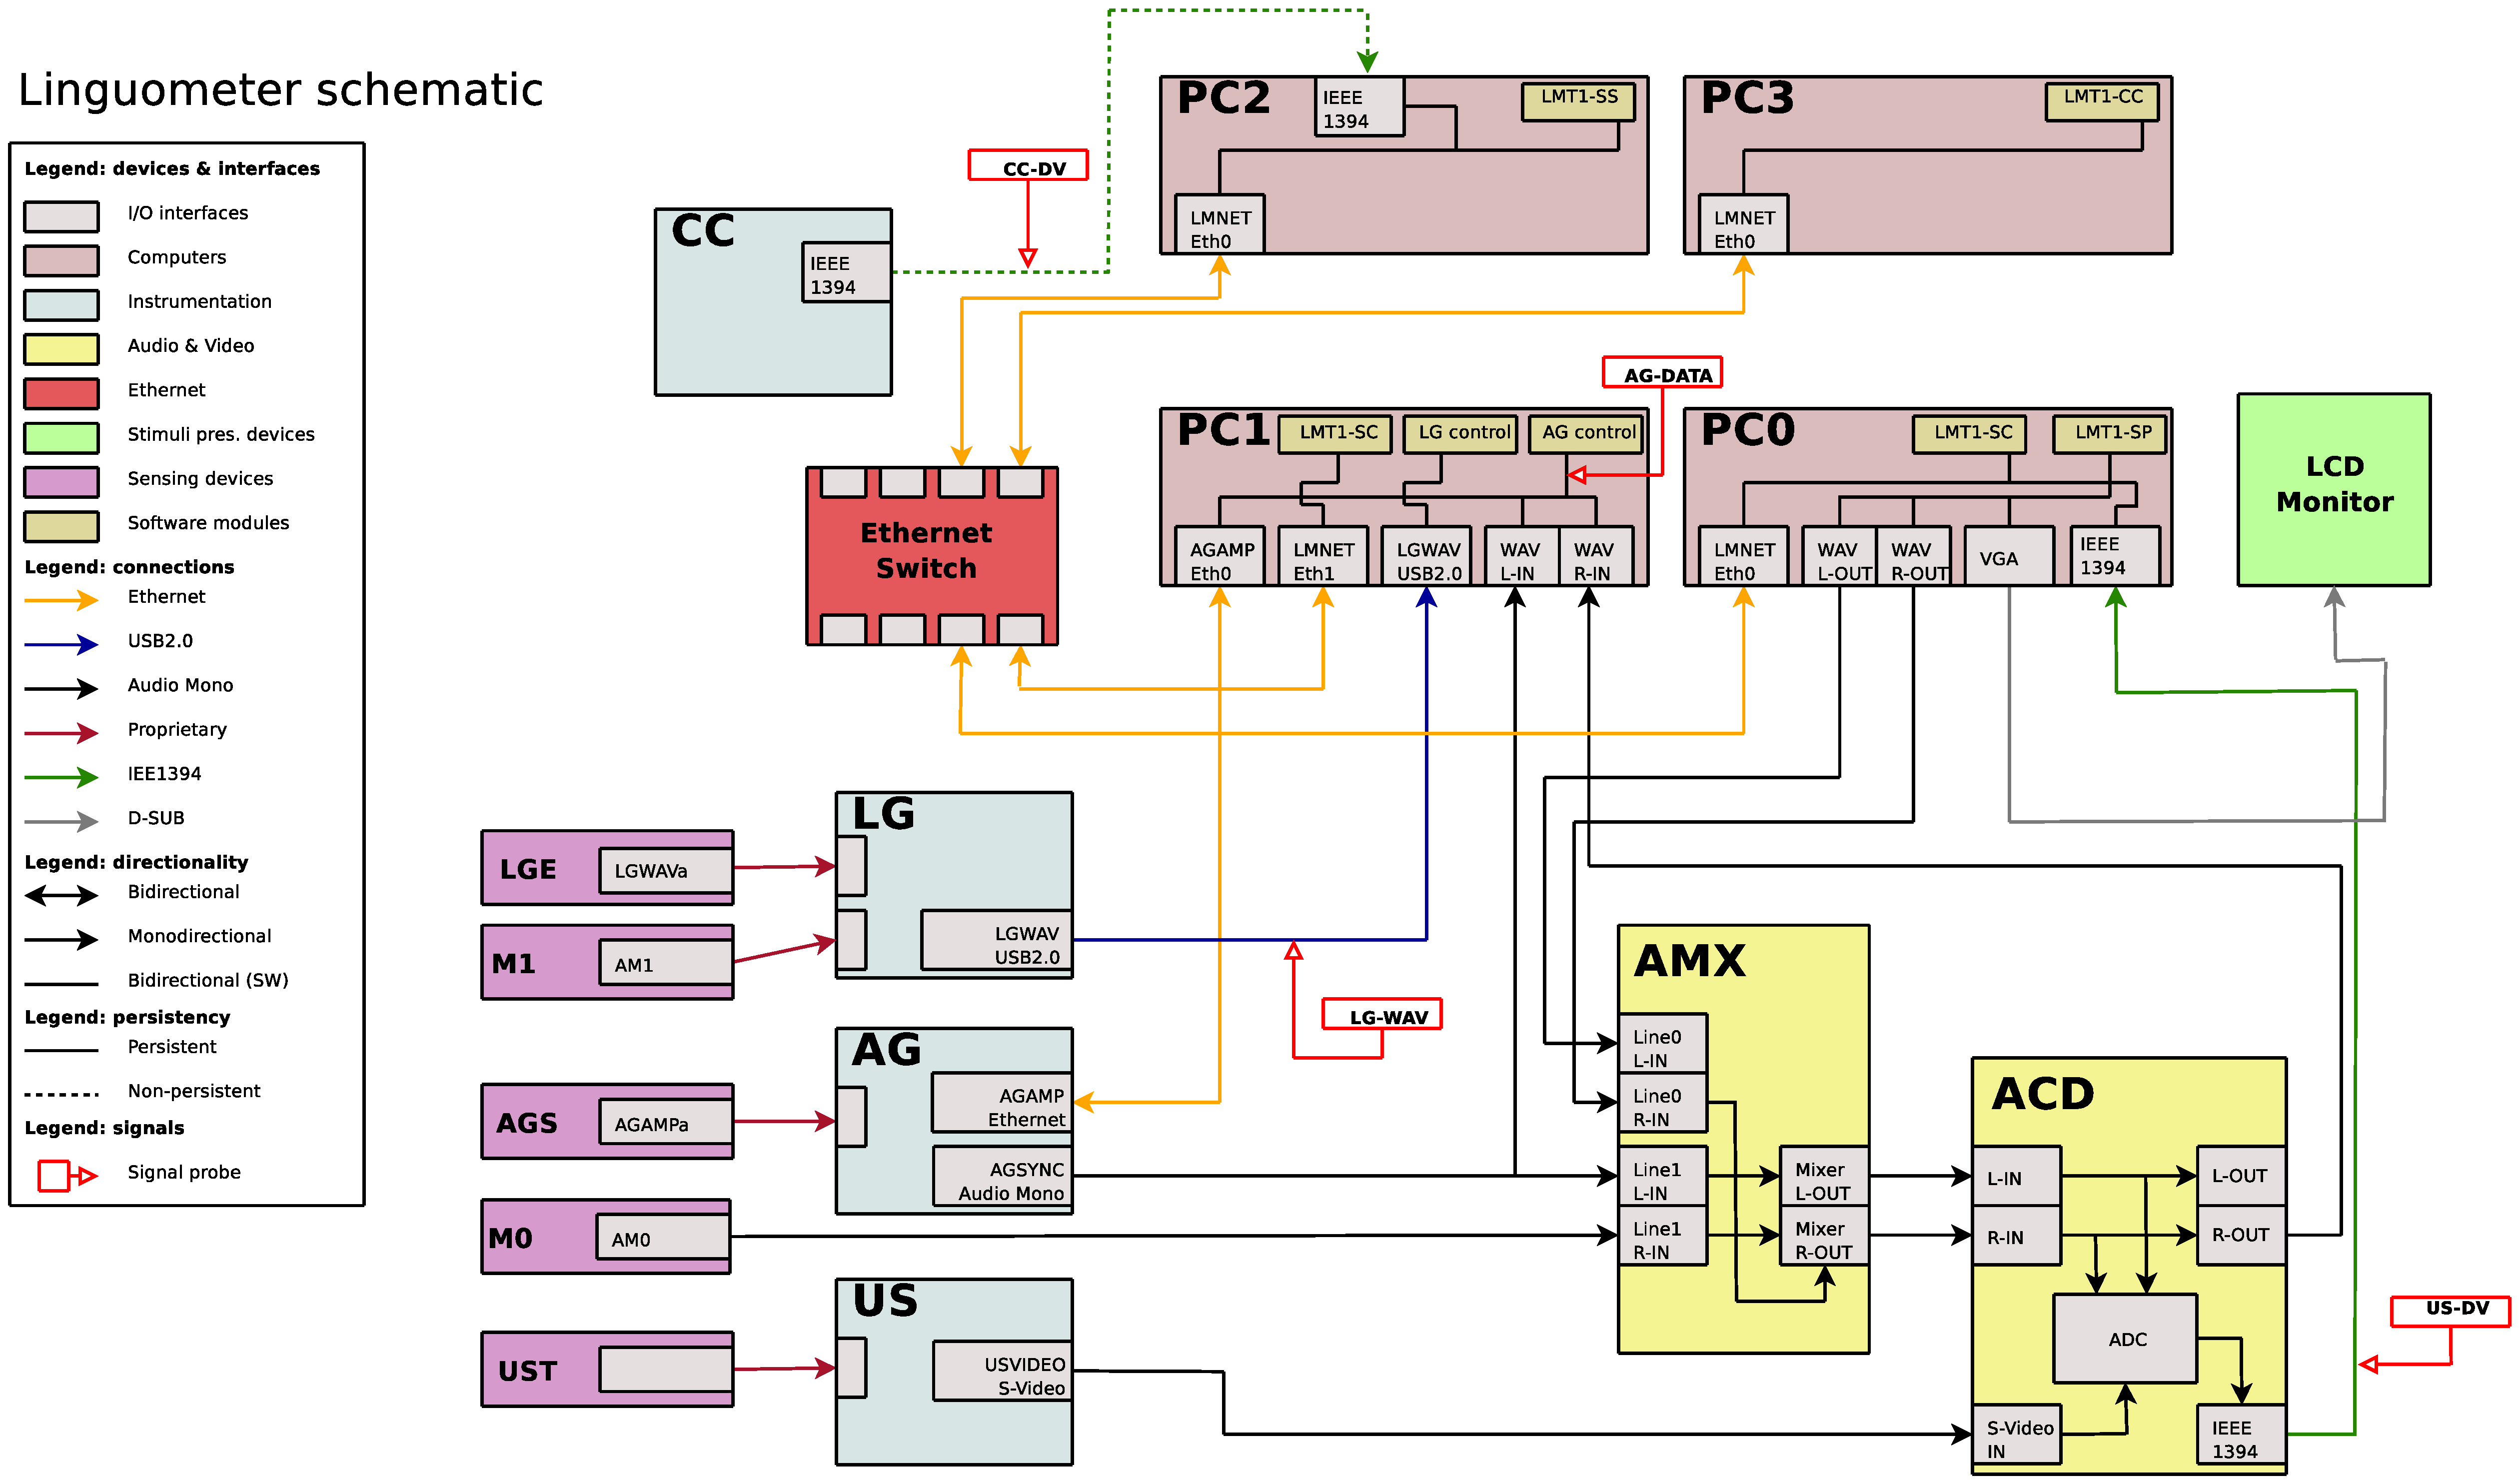
\epsfig{file=include/linguometer/images/schematics.eps,width=0.90\textwidth}
	\caption[Linguometer schematic diagram]{\textbf{Linguometer schematic diagram
	}: the diagram shows the building blocks onto which the Linguometer is
	integrated and their connections. Please refer to
	Section~\ref{sec:linguometer:architecture:diagram} for a detailed
	description of the building-blocks and connections.}
	\label{fig:linguometer:architecture:schematics}
\end{sidewaysfigure}
% ---------------------------------------------------------------------------- %


As previously said, the workflow diagram highlights the instants in which the
experimenters start/stop a particular recording device.
In this perspective, the camcorder is the first device to start recording,
followed by the ultrasound system, the laryngograph and the articulograph.
When all the devices are recording, the stimuli are submitted via 
the \emph{lmwords} program so that the first and the second word are then 
sequentially displayed onto the screen and read by the subject.
Stimuli submission did require an experimenter to check if the word was
pronounced incorrectly and 
eventually mark the word to be submitted again at the
end of the batch.
At the beginning of a batch of stimuli (\tstart{WD}) and at its end 
(\tstop{WD}), \emph{lmwords} produces two different segmentation signals.
In the same way, each word is delimited by two analogue signals 
(e.g.: \tstarti{WD}{0} and \tstopi{WD}{0}).
At the bottom of Figure~\ref{fig:linguometer:architecture:workflow}, 
the legend shows the symbolic waveform adopted for such signals (word batch
start/stop and word start/stop).
Those signals, routed to the \sig{AMX} mixer and mixed with the main speech
signal \sig{AM0}, are largely used in post processing to automatically align 
and segment the dataset.

Dr. M. Ferro\footnote{NEUROLAB, Universit\`a di Ferrara, Ferrara, Italy.} lead
the stimuli submission protocol while M. Tavella controlled the
setup, starting and stopping the devices as shown in the workflow diagram.
Once the stimuli have been submitted, the recording devices shutdown procedure
starts.
The first device to be stopped is \wf{AG}, followed by \wf{LG}, \wf{US} and
\wf{CC}.

% ---------------------------------------------------------------------------- %
\begin{figure}%[!ht]
\centering
\epsfig{file=include/linguometer/images/workflow.eps,width=0.90\textwidth}
	\caption[Linguometer workflow diagram]{\textbf{Linguometer workflow
	diagram}: 
	the Linguometer schematic is extensively used to represent the ``spatial'' 
	organization of the Linguometer 
	(Figure~\ref{fig:linguometer:architecture:schematics}).
	The previous representation describes the
	connections used to integrate the setup, although it lacks of explanations
	from the temporal point of view.
	Sharing the same device representation with the Linguometer schematic,
	the workflow diagram describes how data is acquired during an experiment.}
	\label{fig:linguometer:architecture:workflow}
\end{figure}
% ---------------------------------------------------------------------------- %

It has been said that the workflow and the data-streams diagrams share the 
same time scale. To stress this relationship, dotted lines and arrows 
are used in Figure~\ref{fig:linguometer:architecture:workflow}.
Each dotted line is used to mark a particular instant in time, pinpointed by a
time label.
The reader surely noticed that the data-streams diagram shows four different 
composite bars: \wf{CC-DV}, \wf{US-DV}, \wf{LG-WAV} and \wf{AG-DATA}.
Each one of those bars provides a simbolic description of the data-streams 
recorded by the \wf{CC}, \wf{US}, \wf{LG} and \wf{AG} devices respectively.
In the following paragraphs, the Linguometer recording mechanism is discussed
considering what happens instant by instant, and linking the data-streams
diagram to the Linguometer block diagram, thus linking the temporal level with
the connection level.

% ---------------------------------------------------------------------------- %
\tstart{CC} - The \sig{CC} camcorder is the first recording device to be
started. 
\sig{CC} records a video stream of the subject's facial experssions
(\wf{CC-Video}) and a stereo audio stream of the subject's speech 
(\wf{CC-SpeechL} and \wf{CC-SpeechR}).
The audio stream is recorded via an embedded microphone not shown in the
schematic diagram.\\

% ---------------------------------------------------------------------------- %
\tstart{US} - The \sig{USVIDEO} stream is acquired by \sig{PC0} via the
\sig{ACD} acquisition
card.
The acquisition card also records a stereo audio signal, in this case the
output of the \sig{AMX} audio mixer.
The \wf{AGSYNC} signal is routed through the mixer (\sig{Line1 L-IN}) to the 
acquisition card (\sig{L-IN}) and is then digitized, becoming the \wf{US-SYNC}
signal.
The synchronization peaks generated by the articulograph via the Sybox-Opto4
device are shown in the data-streams diagram
(Legend: \emph{AG sweep start/stop}).
Similarly, the speech signal \sig{AM0} sensed by the \sig{M0} microphone is
routed to \sig{Line1 R-IN} and mixed with the segmentation signal generated 
by \sig{PC0} via \emph{lmwords}.
This last signal reaches the \sig{AMX} mixer at the level of the \sig{Line0}
stereo input.
The mixed signal is digitized and is labeled \wf{US-Speech} in the workflow
diagram.
The \wf{US-Speech} stream shows two components: the word waveforms (word 0 and
word 1, in the Legend) and the segmentation signals (\emph{word start/stop} and 
\emph{word batch start/stop}).
The first component is the digitized version of the \sig{AM0} speech signal,
and its replicas are shown in the \wf{CC-DV}, \wf{LG-WAV} and \wf{AG-Speech}
streams\footnote{For the sake of simplicity, the different replicas are shown
with identical symbols. In reality, the replicas are not identical 
(they differ since different microphones and devices are used in the 
acquisition process), although their waveforms are very similar.}.
The latter component is the digitized version of the segmentation signals
generated by the \emph{lmwords} stimuli presentation program
(\sig{LMT1-SP}).
Once digitized, the \wf{AG-Speech} signal leaves the \sig{ACD} acquisition
card and it is routed to the right channel of the \sig{PC1} computer sound card
(\sig{WAV R-IN}), thus becoming the \wf{AG-Speech} signal.
As discussed in Section~\ref{sec:linguometer:architecture:blocks}, the AG500
articulograph control software (\sig{AG control}) records the amplitudes of the
sensors and the speech signal synchronously, after the \sig{AGSYNC} signal is
detected.
The \wf{US-DV} stream is the core of the hardware synchronization mechanism. 
In fact, the ultrasonographic video stream is recorded synchronously with the
articulograph synchronization signal.
As a result, finding the \emph{AG sweep start/stop} signals in \wf{US-Sync} 
allows the alignment of the ultrasonographic video stream to the articulographic 
data.
Once the \sig{AG} and the \sig{US} data-streams are synchronized, it is possible
to align the \wf{CC-Video} and the \wf{LG-EGG} streams simply by aligning
\wf{CC-SpeechL} (or \wf{CC-SpeechR}) and \wf{LG-Speech} to
\wf{US-Speech}.\\

% ---------------------------------------------------------------------------- %
\tstart{LG} - The \sig{LG} laryngograph is started. 
The \sig{PC1} control PC acquires the \wf{LG-WAV} stereo stream. 
\wf{LG-Speech} corresponds to a digitiez version of the \sig{AM1}
signal sensed via the \sig{M1} microphone.
On the other hand, \wf{LG-EGG} is the digitized version of the signal acquired
via the laryngograph electrodes.\\

% ---------------------------------------------------------------------------- %
\tstart{AG} - The \sig{AG} recording sweep is started.
The \sig{AGSYNC} synchronization signal is sent both to the \sig{AG control}
software and to the \sig{AMX}-\sig{ACD} blocks.
Once the \sig{AG control} program detects the \emph{AG sweep start} signal, it
starts acquiring the \wf{AG-DATA} stream.
The \emph{AG sweep start} synchronization signal is also present in the
\wf{US-Sync} stream and it is used in post-processing to align the
articulographic and the ultrasonograpic data.\\

% ---------------------------------------------------------------------------- %
\tstart{WD} - An experimenter, pressing a key on the \sig{PC0} computer,
generates the \emph{Word batch start} segmentation signal.
The \sig{PC0} sound card is connected to the \sig{AMX} mixer, and the
segmentation signals are mixed with the speech signal \sig{AM0}.
Since the \sig{AMX} output is connected to \sig{ACD} input, the mixed
signal is acquired by \sig{ACD} and then routed to \sig{PC1}, where it is also
acquired by \sig{AG control}.
The \emph{Word batch start} signal is visible both in the \wf{AG-Speech} and in
the \wf{US-Speech} tracks.
The segmentation signals that identifty the beginning (and the end) of a batch
of stimuli, are used in post-processing to align and segment the dataset.
Since the \emph{Word start}, the \emph{Word stop} and the \emph{Word batch stop}
signals follow exactly the same route here discussed for \emph{Word batch
stop}, similar descriptions are omitted in the following paragraphs.\\

% ---------------------------------------------------------------------------- %
\tstarti{WD}{0} - An experimenter, pressing a key on the \sig{PC0} computer, 
generates the  \emph{Word start} segmentation signal and displays a stimulus
on the LCD screen (in this case \emph{Word 0}).
The per-word segmentation signals play an important role in post-processing,
mainly for segmentation and alignment.
The reader should have noticed that, on the onset of speech, all the Linguometer
devices are simultaneously acquiring a large and differentiated set of 
phono-articulatory features.\\

% ---------------------------------------------------------------------------- %
\tstopi{WD}{0} - An experimenter, pressing a key on the \sig{PC0} computer, 
marks the word as pronounced correctly or uncorrecly, generates the
\emph{word stop}
segmentation signal and finally moves to the next stimuli.
The interval of time between \tstopi{WD}{0} and \tstarti{WD}{1} is not handled
by the experimenter, but is coded inside
\emph{lmwords}\footnote{The interval between two words lasts 750 ms and is
used in post processing to verify if the acquired audio signals are affected by 
drift.}.\\

% ---------------------------------------------------------------------------- %
\tstarti{WD}{1} and \tstopi{WD}{1} - The experimenter presents the second 
stimuli.\\

% ---------------------------------------------------------------------------- %
\tstop{WD} - The \emph{lmwords} program detects that no more stimuli need to be 
submitted to the subject, generates the \emph{word batch stop} segmentation
signal
and finally quits.\\

% ---------------------------------------------------------------------------- %
\tstop{AG} - The experimenter stops recording with the articulograph AG500. 
The Sybox-Opto4 synchronization device generates the \emph{AG sweep stop}
synchronization signal, visible in the \wf{US-Sync} track.\\

% ---------------------------------------------------------------------------- %
\tstop{LG}, \tstop{US} and \tstop{CC} - The experimenter turns off the
laryngograph,
the acquisition card and the
camcorder.\\
% ---------------------------------------------------------------------------- %

The reader surely noticed that the audio mixer and the acquisition card play a
crucial role in the Linguometer synchronization mechanism.
In fact, the \wf{US-DV} stream contains enough information to align the sagittal
reconstruction of tongue motion recorded by the means of ultrasonography with 
the kinesthetic information derived from the articulographic investigation.
To sum up, ultrasonographic and speech data are synchronized in hardware
(\wf{US-Video} and \wf{US-Speech}).
The amplitudes recorded with the articulograph, from which the kinesthetic
informations are derived, are synchronized with the \wf{US-Video}/\wf{US-Speech}
streams since the \sig{AGSYNC} signal is known and it is also acquired
simultaneously with the previous signals (\wf{US-Sync}).
The~\wf{US-Speech} signal provides a reference for aligning other sources of
phono-articulatory information, such as the laryngographic data and the facial
expressions data.
As a matter of fact, it was not possible to route the segmentation and the
synchronization signals on the camcorder and the laryngograph, since those
devices required the use of a stand-alone microphone\footnote{The microProcessor by 
Laryngograph Ltd can acquire a
further stereo audio signal at line level, although the sampling rate of the
Lx/Gx signals decreases from 16kHz to 12kHz~(Xinghui Hu, Laryngograph Ltd.
Private communication).}.
The \wf{LG-WAV} and the \wf{CC-DV} signals are initially segmented and
then each word is aligned, by means of cross-correlation, with the words 
extracted from the \wf{US-Speech} stream. The alignment/segmentation process
is better described in Section~\ref{ch:results}.
% ---------------------------------------------------------------------------- %
\pagebreak
% ---------------------------------------------------------------------------- %
